\documentclass[11pt]{article}
\usepackage[utf8]{inputenc}
\usepackage[T1]{fontenc}
\usepackage[spanish]{babel}
\usepackage{lmodern}
\usepackage[margin=1in]{geometry}
\usepackage{hyperref}
\usepackage{amsmath,amssymb}
\usepackage{booktabs}
\usepackage{array}
\usepackage{graphicx}
\usepackage{xcolor}
\graphicspath{{figures/}}
\emergencystretch=3em

\definecolor{vermil}{HTML}{D55E00}
\definecolor{recgreen}{HTML}{009E73}
\definecolor{stdblue}{HTML}{0072B2}

% Keep decimal points (not Spanish decimal commas) so every number here
% matches the English manuscript and code artifacts exactly.
\decimalpoint

\title{Diseño del Espacio de Acciones en el Benchmark DES/RL Fundamentado en Garrido:\\
Qué Cambiamos, Por Qué, y Qué Produjo}
\author{}
\date{}

\begin{document}
\maketitle

\begin{abstract}
\noindent Esta nota documenta, con precisión y con trazabilidad completa
al código y a los datos, las decisiones de diseño del espacio de acciones
detrás de los dos carriles experimentales de nuestro benchmark de
aprendizaje por refuerzo sobre el modelo de cadena de suministro de
alimentos militar (MFSC) de Garrido-Rios (2017). Responde tres preguntas
directamente: (1) qué contrato de acciones usamos realmente, y cómo se
relaciona con el diseño discreto original de Garrido de buffer/turno; (2)
por qué las políticas aprendidas resultantes no lograron superar a la
mejor política estática bajo el alcance de decisión original (Track A); y
(3) qué extensión logró que una política aprendida ganara, y por qué
creemos ese resultado. Cada número citado aquí traza a un artefacto
fechado en el repositorio del proyecto; ninguno es ilustrativo.
\end{abstract}

\section{Propósito}

La tesis de Garrido-Rios estudia dos familias de decisión para el MFSC:
buffers de inventario estratégicos en tres puntos de la cadena (Op3, Op5,
Op9) y capacidad de manufactura de corto plazo mediante turnos de
ensamble. Ambas se variaron de forma \emph{discreta} y \emph{un factor a
la vez} en el diseño de experimentos (DOE) original. Nuestra propuesta
inicial --- comunicada directamente a Garrido --- fue que esta grilla de
diseño de experimentos podía reemplazarse por una parametrización
continua mucho más pequeña: una variable continua de buffer y una
variable de turno (efectivamente discreta, de tres niveles), en lugar de
las 15 configuraciones de buffer y 3 niveles de turno originales
examinados por separado. Esta nota explica exactamente qué construimos a
partir de esa idea, qué ocurrió al entrenar una política aprendida sobre
ella, por qué no ganó, y qué cambiamos después para obtener una victoria
genuina y robustamente probada.

\section{Las variables de decisión originales de Garrido-Rios}
\label{sec:garrido}

La Tabla~\ref{tab:garrido_design} resume el diseño de la tesis (Capítulo
6, Escenarios II--III). Tres ubicaciones (Op3: almacén de materia prima,
Op5: buffer de pre-ensamble, Op9: batallón de suministro de raciones)
pueden cada una mantener un buffer de inventario estratégico, reabastecido
en uno de cinco intervalos fijos. Por separado, la línea de ensamble puede
operar en uno de tres niveles de turno. Las dos familias nunca se variaron
conjuntamente: el Escenario II fija $S=1$ y varía los niveles de buffer
(configuraciones Cf31--Cf60); el Escenario III fija el buffer en cero y
varía el nivel de turno (Cf61--Cf90). Este es un DOE válido y eficiente,
un factor a la vez, para un estudio de simulación de eventos discretos,
pero significa que la tesis nunca observó directamente qué ocurre cuando
buffer y turno se ajustan juntos, y nunca expresó ninguna de las dos
variables en una escala continua.

\begin{table}[htbp]
\centering
\caption{Diseño de buffer/turno de Garrido-Rios (2017) (Tablas 6.16,
6.20--6.23). Cantidades de buffer en unidades de raciones/materia prima;
intervalo en horas.}
\label{tab:garrido_design}
\small
\begin{tabular}{lccccc}
\toprule
Intervalo (h) & 168 & 336 & 504 & 672 & 1{,}344 \\
\midrule
Op3 (materia prima) & 15{,}360 & 30{,}720 & 46{,}080 & 61{,}440 & 122{,}880 \\
Op5 (pre-ensamble) & 15{,}360 & 30{,}720 & 46{,}080 & 61{,}440 & 122{,}880 \\
Op9 (raciones) & 15{,}750 & 31{,}500 & 47{,}250 & 63{,}000 & 126{,}000 \\
\bottomrule
\end{tabular}

\vspace{0.4em}
\begin{tabular}{lccc}
\toprule
Nivel de turno $S$ & 1 & 2 & 3 \\
\midrule
Capacidad anual (raciones) & 738{,}432 & 1{,}476{,}864 & 2{,}215{,}296 \\
\bottomrule
\end{tabular}
\end{table}

Esto da $3 \times 5 = 15$ configuraciones discretas de buffer y 3 niveles
discretos de turno --- los ``15 buffers y 3 turnos'' a los que nos
referimos en nuestra conversación con Garrido --- examinados un factor a
la vez (30 configuraciones de buffer a través de los dos bloques de
réplica/riesgo, más 30 configuraciones de turno, Cf31--Cf90 en la
numeración de la tesis).

\section{De la grilla de Garrido a un espacio de acciones entrenable}
\label{sec:reduction}

Un agente de aprendizaje por refuerzo necesita una interfaz de acciones
diferenciable y de baja cardinalidad; entrenar directamente sobre la
grilla de 15 celdas de buffer de Garrido (o peor, la grilla conjunta
completa de $15 \times 3 = 45$ celdas que él nunca pobló) dejaría a un
método de gradiente de política sin señal útil entre puntos de la grilla.
La reducción que propusimos a Garrido, y el refinamiento posterior que
hicimos tras probarla, procedió en tres pasos (Figura~\ref{fig:chain}).

\begin{figure}[htbp]
\centering
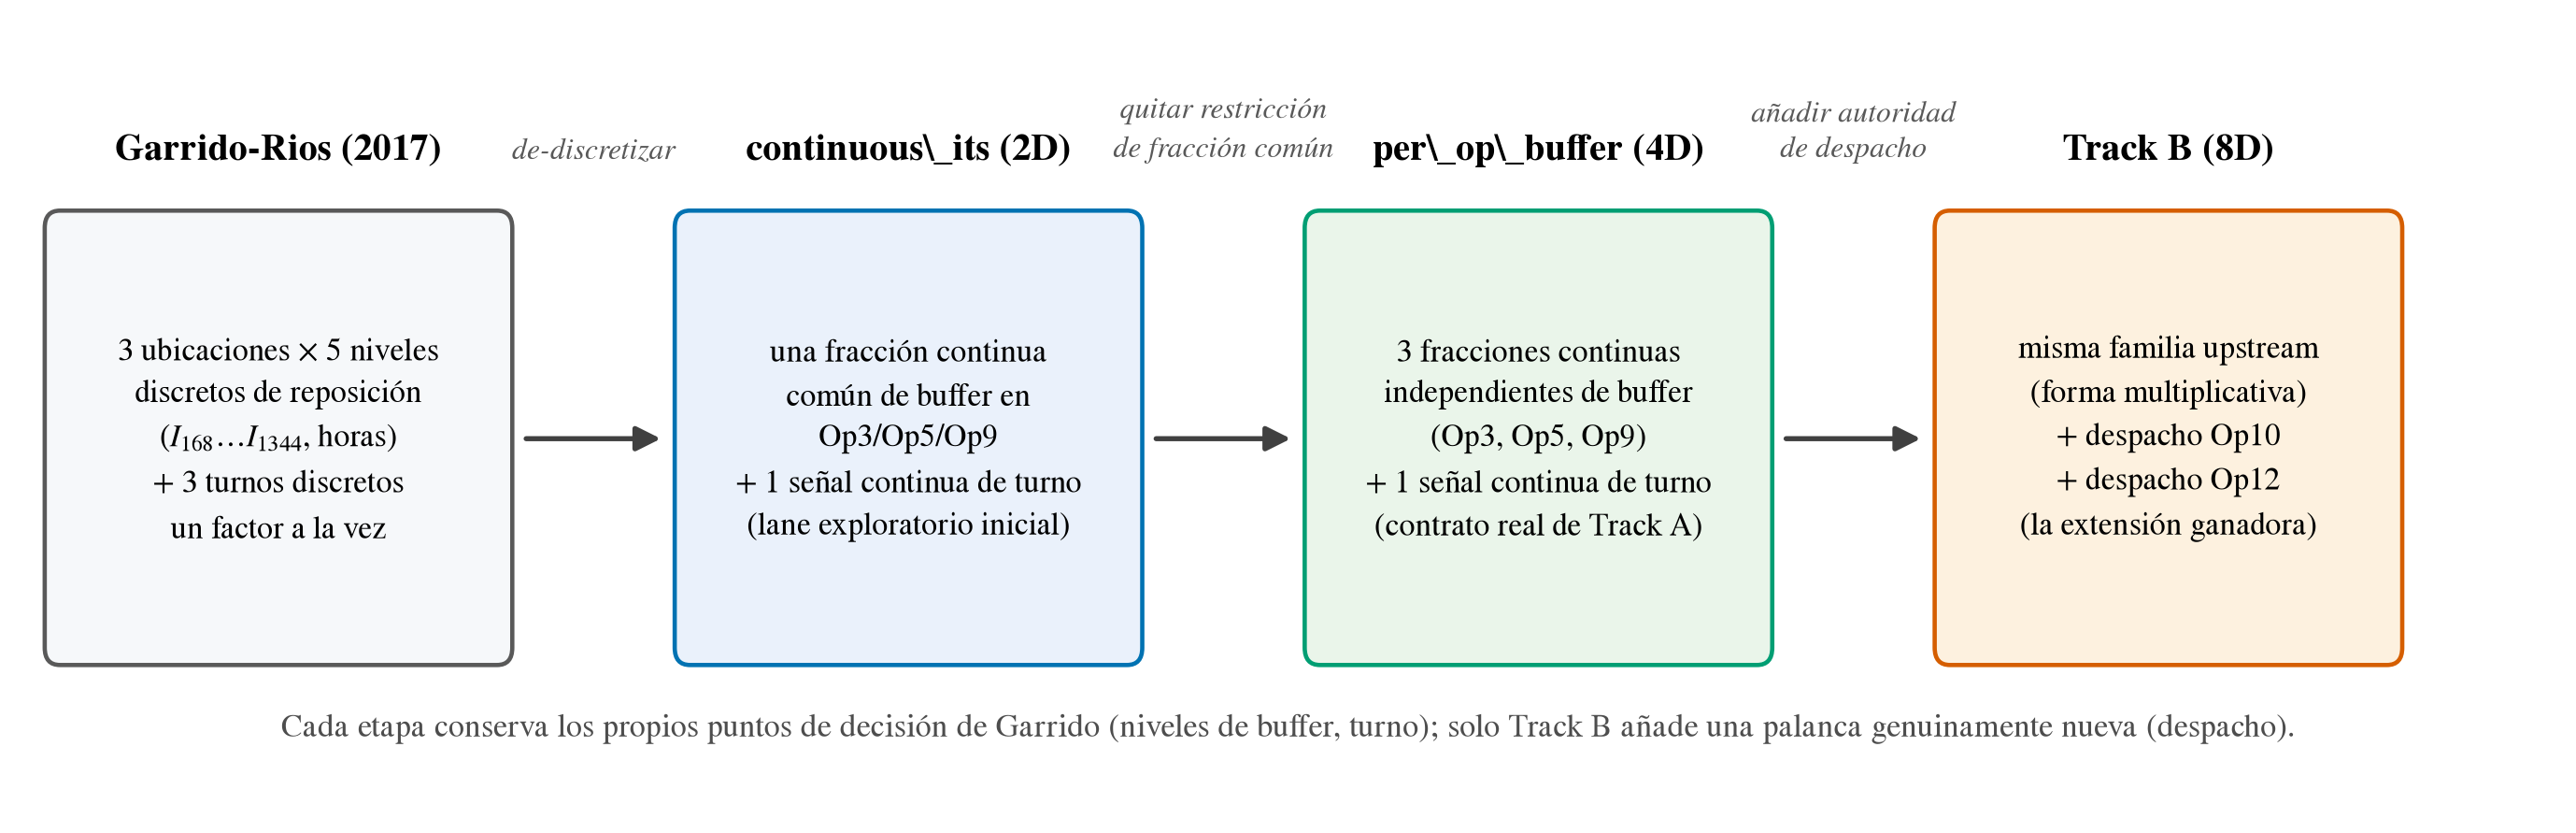
\includegraphics[width=\linewidth]{fig_reduction_chain}
\caption{La cadena de reducción del espacio de acciones realmente
implementada, desde el diseño de experimentos discreto de Garrido hasta
los dos carriles experimentales del paper. Cada etapa conserva los propios
puntos de decisión de Garrido; solo la etapa final (Track B) añade una
palanca genuinamente nueva.}
\label{fig:chain}
\end{figure}

\subsection{Paso 1: \texttt{continuous\_its} --- la idea que propusimos}

Nuestra primera implementación (\texttt{continuous\_its\_env.py},
contrato \texttt{track\_a\_continuous\_its\_v1}) es exactamente la simplificación
descrita a Garrido: un único escalar continuo $f \in [0,1]$, que
representa la fracción del nivel de buffer más grande ($I_{1{,}344}$)
aplicada \emph{en común} a Op3, Op5 y Op9 simultáneamente, más una única
señal continua de turno mapeada mediante umbrales fijos a
$S \in \{1,2,3\}$. Este es un espacio de acciones genuinamente
bidimensional: un dial de buffer, un dial de turno. Un tamizaje temprano a
pequeña escala (2 semillas de entrenamiento) mostró una señal adaptativa
prometedora en Excel ReT y CVaR, pero una repetición confirmatoria de 3
semillas y una evaluación posterior de números aleatorios comunes (CRN)
densa contra una frontera estática equivalente fallaron en reproducirla:
la aparente victoria no sobrevivió una comparación estática más densa y
justa. Registramos esto honestamente como un carril exploratorio no
confirmado y superado, no como evidencia a favor ni en contra de la
afirmación central.

\subsection{Paso 2: \texttt{per\_op\_buffer} --- el contrato real de Track A}

La fracción única y compartida de buffer del Paso 1 tiene una limitación
real: obliga a la política a subir o bajar el inventario en Op3, Op5 y Op9
en conjunto, aun cuando el propio diseño de Garrido trata estos puntos
como tres decisiones independientes. Eliminamos esta restricción
(\texttt{supply\_chain/continuous\_its\_env.py}, clase
\texttt{PerOpBufferTrackAEnv}, contrato
\texttt{track\_a\_per\_op\_buffer\_v1}): el espacio de acciones se
convierte en
\begin{equation}
a = (f_{\mathrm{Op3}},\, f_{\mathrm{Op5}},\, f_{\mathrm{Op9}},\, s) \in [0,1]^3 \times [-1,1],
\end{equation}
tres fracciones continuas independientes de buffer objetivo (cada una
expresada aún en relación con la propia escala $I_{1{,}344}$ de Garrido de
la Tabla~\ref{tab:garrido_design}) más una señal continua de turno ---
cuatro dimensiones en total. Este es el contrato realmente usado para el
resultado principal de Track A en el paper (Sección~\ref{sec:tracka}): es
estrictamente más rico que la versión de fracción compartida, y preserva
cada uno de los puntos de decisión propios de Garrido mientras elimina
tanto su discretización en cinco niveles fijos \emph{como} la restricción
de un factor a la vez (buffer y turno ahora pueden moverse juntos
libremente). La Tabla~\ref{tab:dof} compara los tres diseños directamente.

\begin{table}[htbp]
\centering
\caption{Grados de libertad: el diseño de Garrido frente a nuestras dos
reducciones continuas.}
\label{tab:dof}
\small
\begin{tabular}{p{0.22\linewidth}p{0.72\linewidth}}
\toprule
Diseño & Variables de decisión \\
\midrule
Garrido-Rios (tesis) & 15 configuraciones discretas de buffer (3
ubicaciones $\times$ 5 niveles) + 3 niveles discretos de turno; variados
un factor a la vez \\
\texttt{continuous\_its} & 1 fracción continua de buffer (compartida entre
las tres ubicaciones) + 1 señal continua de turno; de-discretizado, pero
las tres ubicaciones no pueden fijarse de forma independiente \\
\texttt{per\_op\_buffer} (Track A) & 3 fracciones continuas independientes
de buffer (Op3, Op5, Op9) + 1 señal continua de turno; granularidad
completa de Garrido preservada, discretización eliminada \\
\bottomrule
\end{tabular}
\end{table}

\section{Track A: por qué la relajación continua tampoco gana}
\label{sec:tracka}

Antes de entrenar cualquier agente, primero preguntamos si el propio
espacio de decisión \emph{estático} contiene estructura explotable: se
compara un oráculo condicionado al régimen (la mejor combinación de
buffer/turno \emph{por régimen de disrupción}) contra la única mejor
política constante independiente del régimen sobre una grilla densa (cinco
familias de riesgo $\times$ cinco multiplicadores de frecuencia $\times$
tres multiplicadores de impacto). El oráculo supera a la mejor política
constante por \textbf{+0.000176 a +0.000296 Excel ReT} (límite inferior
del IC del 95\% positivo) --- un margen pequeño pero genuino y distinto de
cero. La pregunta relevante es si una política aprendida puede capturarlo.

Ninguno de los agentes probados lo logra. Probamos PPO continuo
directamente sobre el contrato \texttt{per\_op\_buffer}, PPO
pre-entrenado mediante clonación de comportamiento sobre la propia tabla
de acciones del oráculo, y PPO entrenado bajo una variante de
conflicto-de-familia del mismo contrato con recompensa
\texttt{ReT\_excel\_plus\_cvar} (5 semillas). El enfoque más cercano ---
PPO pre-entrenado por clonación de comportamiento --- falla en igualar al
mejor comparador estático por
\[
-6.99\times10^{-6}\ \text{Excel ReT} \quad (0.155247\ \text{vs.}\ 0.155254),
\]
una brecha dos órdenes de magnitud menor que el margen de oráculo medido,
y está Pareto-dominado por diez configuraciones estáticas en la frontera
conjunta de Excel ReT/recurso (Tabla~\ref{tab:tracka}).

\begin{table}[htbp]
\centering
\caption{Resumen de frontera de Track A. Los valores son Excel ReT bajo la
familia de evaluación de Track A; el margen del oráculo usa la misma
métrica.}
\label{tab:tracka}
\small
\begin{tabular}{p{0.28\linewidth}p{0.14\linewidth}p{0.16\linewidth}p{0.28\linewidth}}
\toprule
Familia de política & Mejor aprendida & Mejor estática & Resultado \\
\midrule
PPO (continuo, reparado) & 0.155247 & 0.155254 & pierde ($-7.0\times10^{-6}$) \\
PPO pre-entrenado por BC & 0.155247 & 0.155254 & pierde; Pareto-dominado \\
Oráculo condicionado al régimen & --- & $+0.000176$ a $+0.000296$ &
margen existe, no convertido \\
\bottomrule
\end{tabular}
\end{table}

\subsection{La razón estructural}

La razón no es que el espacio de decisión buffer/turno esté mal
parametrizado. Es que la decisión que controla el agente no es la
restricción que gobierna la recuperación. La Figura~\ref{fig:topology}
marca el cuello de botella vinculante directamente sobre la topología del
MFSC: el rendimiento de transporte aguas abajo en Op10 y Op12 (despacho de
línea de comunicación hacia las unidades de apoyo de servicio de combate y
de ahí al teatro) opera en aproximadamente 2{,}400--2{,}600 raciones/día
--- esencialmente igual a la demanda. Una vez que hay un buffer modesto en
su lugar, inventario adicional aguas arriba o capacidad adicional de línea
de ensamble desde un nivel de turno más alto no pueden aumentar lo que
realmente llega al teatro, porque la tubería aguas abajo ya opera cerca de
su techo. Las palancas de buffer y turno, sin importar cuán finamente se
parametricen, se ubican enteramente aguas arriba de esta restricción. Esta
es una instancia directa del principio de la Teoría de Restricciones: el
rendimiento del sistema está gobernado por su restricción vinculante, no
por la mejora del caso promedio en otro punto de la cadena --- y explica
por qué \emph{toda} parametrización probada de la familia buffer/turno
(discreta, continua de fracción compartida, y continua por operación)
converge al mismo resultado negativo.

\begin{figure}[htbp]
\centering
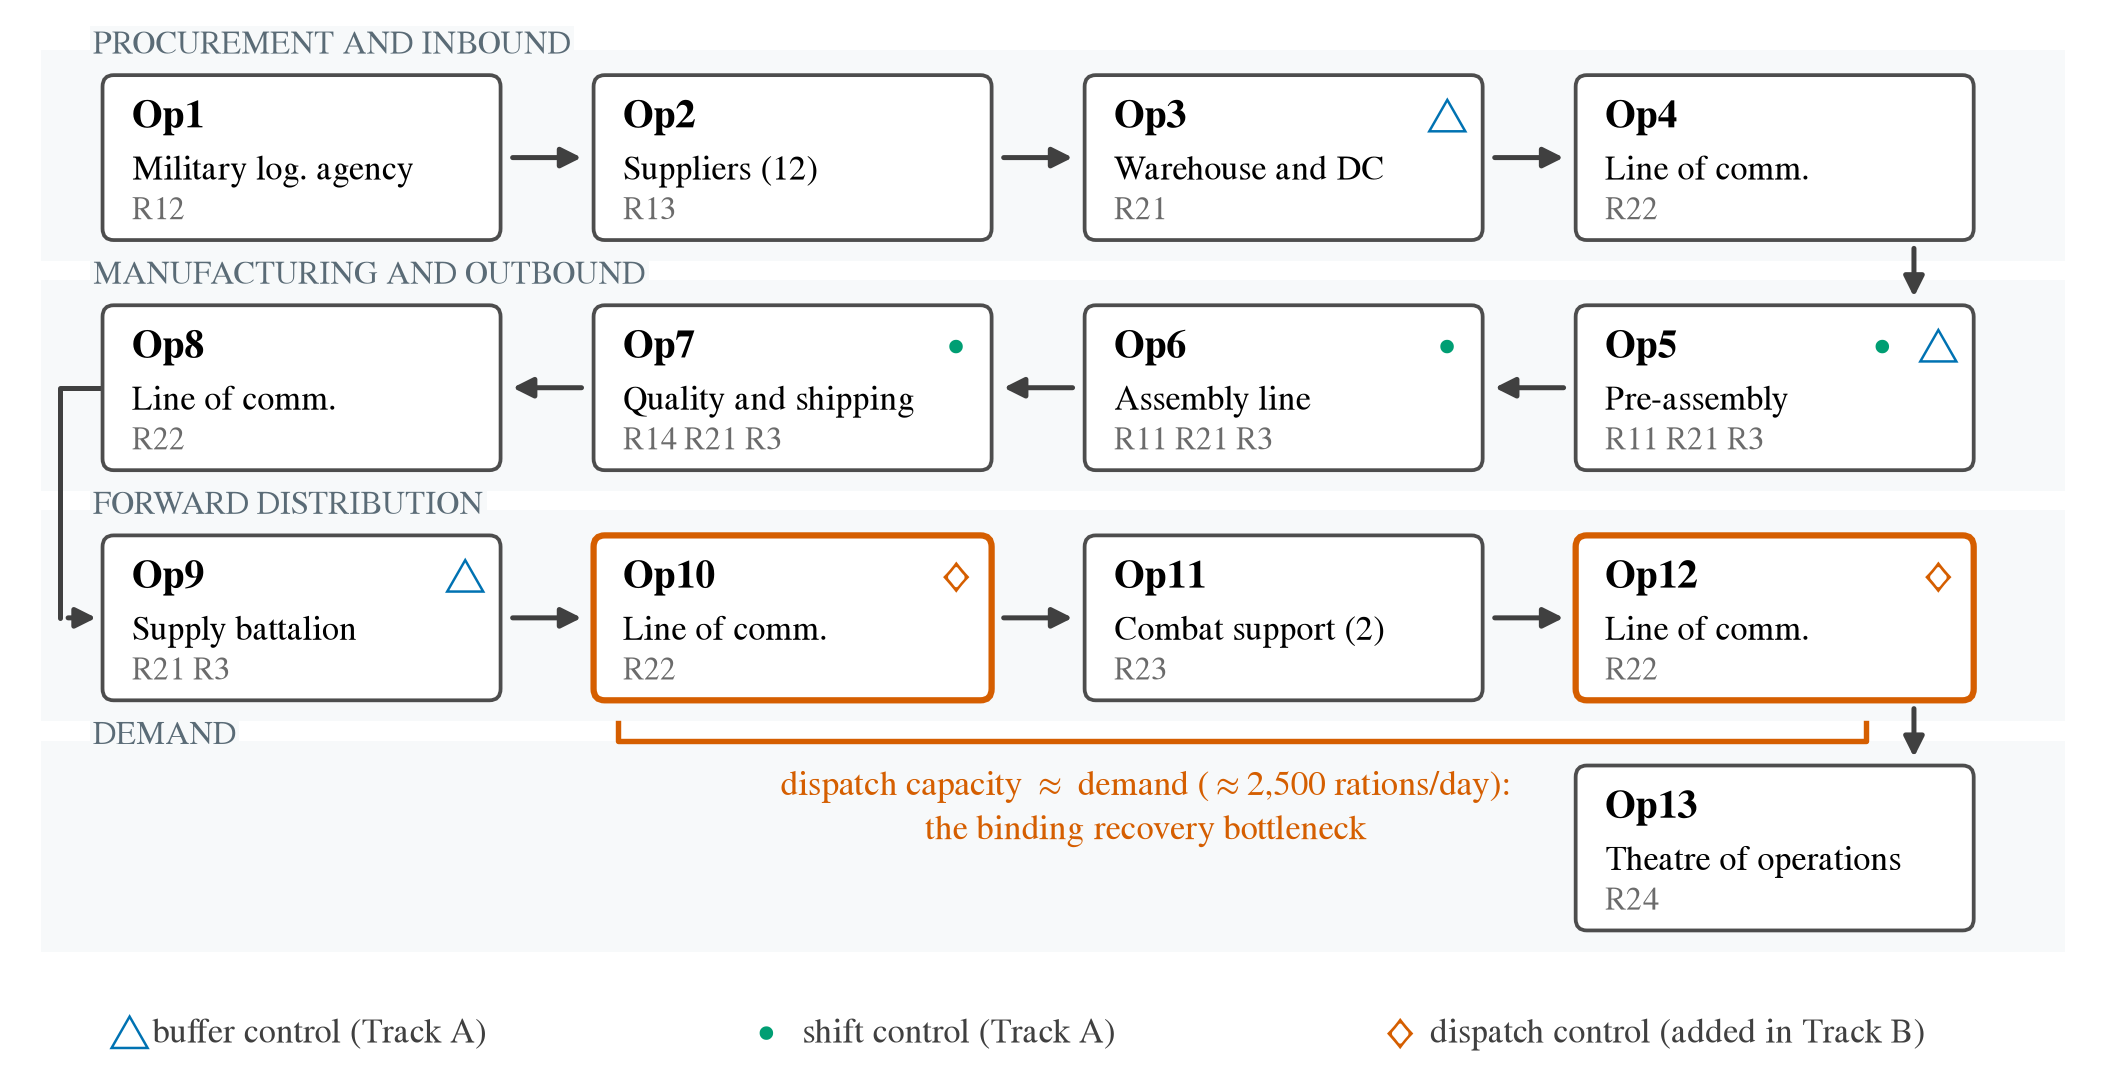
\includegraphics[width=\linewidth]{fig2_mfsc_topology}
\caption{La topología del MFSC con la superficie de control de Track A
(buffer $\bigtriangleup$, turno $\bullet$) y la adición de Track B
(despacho $\diamondsuit$, Op10/Op12) marcadas directamente sobre las
operaciones en las que actúan. El corchete marca el cuello de botella
vinculante de recuperación: la capacidad de despacho aguas abajo iguala
aproximadamente a la demanda. (Figura reproducida del manuscrito en
inglés; las etiquetas se mantienen en el idioma original de envío.)}
\label{fig:topology}
\end{figure}

\section{Track B: añadiendo la única palanca que alcanza el cuello de botella}
\label{sec:trackb}

Track B conserva cada variable de decisión de Track A y añade exactamente
la palanca que la Sección~\ref{sec:tracka} identifica como faltante:
autoridad de despacho de transporte en Op10 y Op12. Para este carril
también cambiamos la parametrización aguas arriba de \emph{fracciones} de
buffer a \emph{multiplicadores} por operación sobre cantidad de pedido y
punto de reorden (una versión más rica, de seis dimensiones, de la misma
familia aguas arriba), de modo que las dos nuevas dimensiones de despacho
pudieran añadirse en la misma forma multiplicativa
(Tabla~\ref{tab:action_contract}). El cambio en la parametrización aguas
arriba no es lo que produce el resultado a continuación --- la
Sección~\ref{sec:tracka} ya mostró que ninguna parametrización de la
familia aguas arriba por sí sola gana --- es una conveniencia de modelado
para adjuntar las dimensiones de despacho de forma consistente.

\begin{table}[htbp]
\centering
\caption{Contrato de acciones \texttt{track\_b\_v1} (8 dimensiones). Las
salidas crudas de la política $x_i \in [-1,1]$ se decodifican por
dimensión; los multiplicadores escalan los parámetros base de la tesis.}
\label{tab:action_contract}
\small
\begin{tabular}{c p{0.32\linewidth} c c}
\toprule
Dim & Variable de decisión & Decodificación & Rango efectivo \\
\midrule
1 & Mult. cantidad de pedido Op3 & $1.25+0.75x$ & $[0.5,2.0]\times 15{,}500$ unid. \\
2 & Mult. cantidad de pedido Op9 & $1.25+0.75x$ & $[0.5,2.0]\times U(2{,}400,2{,}600)$ \\
3 & Mult. punto de reorden Op3 & $1.25+0.75x$ & $[0.5,2.0]\times 168$ h \\
4 & Mult. punto de reorden Op9 & $1.25+0.75x$ & $[0.5,2.0]\times 24$ h \\
5 & Mult. cant. pre-ensamble Op5 & $1.0+0.5x$ & $[0.5,1.5]$ \\
6 & Turnos de ensamble $s_t$ & umbrales en $\pm\tfrac13$ & $\{1,2,3\}$ \\
\textbf{7} & \textbf{Mult. despacho Op10} & $1.25+0.75x$ & $[0.5,2.0]\times U(2{,}400,2{,}600)$ \\
\textbf{8} & \textbf{Mult. despacho Op12} & $1.25+0.75x$ & $[0.5,2.0]\times U(2{,}400,2{,}600)$ \\
\bottomrule
\end{tabular}
\end{table}

\subsection{Resultado}

Bajo el protocolo confirmatorio canónico (10 semillas de entrenamiento,
60{,}000 pasos de tiempo cada una, 12 episodios de evaluación CRN por
semilla, comparado contra la mejor de 147 configuraciones estáticas
densas de despacho), PPO mejora el Excel ReT en
\[
+0.000438\ \text{(Excel ReT }0.005898\text{ vs.\ }0.005460\text{)},
\qquad \text{IC 95\% } [+0.000409, +0.000468],
\]
con las diez medias por semilla individualmente positivas. La misma
política también produce ganancias de magnitud mucho mayor en tasa de
llenado de flujo (0.961 vs.\ 0.669), el tiempo de ciclo de la cola de
recuperación $CT_j$ p99 (1{,}207\,h vs.\ 8{,}113\,h), y el AUC de pérdida
de servicio (una reducción de un orden de magnitud). La
Figura~\ref{fig:pareto} muestra la política en relación con toda la
familia estática de despacho: no es una victoria estricta en costo, pero
domina cada una de las 147 configuraciones estáticas en la frontera
conjunta de resiliencia/cola de recuperación.

\begin{figure}[htbp]
\centering
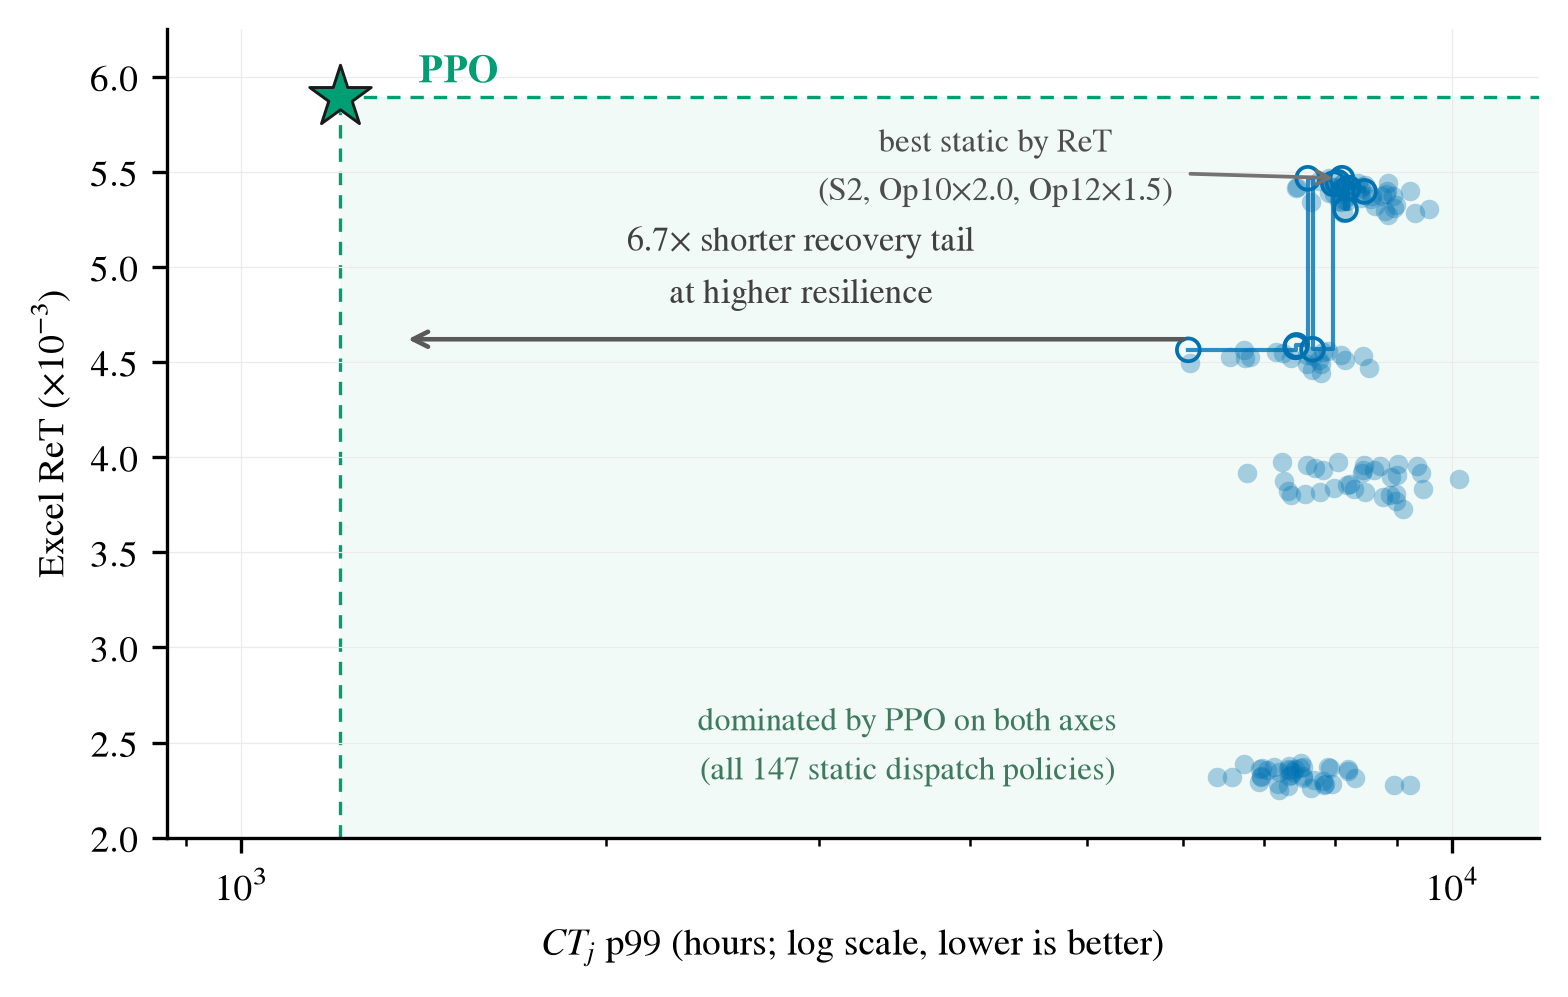
\includegraphics[width=0.85\linewidth]{fig4_pareto_ret_tail_ctj}
\caption{Compensación ReT--cola de Track B, protocolo CRN canónico. PPO
(estrella) domina a toda la familia de 147 políticas estáticas de
despacho simultáneamente en Excel ReT y en la cola de recuperación $CT_j$
p99. (Figura reproducida del manuscrito en inglés.)}
\label{fig:pareto}
\end{figure}

\section{Por qué creemos este resultado}

La victoria de Track B no se acepta solo por la fuerza del número
principal. Se ejecutaron cuatro chequeos adversariales independientes,
diseñados específicamente para descartar las explicaciones alternativas
más comunes de una victoria de RL en un entorno simulado, y los cuatro son
consistentes con que la victoria sea genuina y atribuible específicamente
a la autoridad de despacho añadida:

\begin{itemize}
\item \textbf{\textquestiondown Más actuadores, no más autoridad?} Una ablación del espacio
de acciones (5 semillas, misma escala) compara el contrato completo de 8D
contra variantes de solo-despacho-aguas-abajo (turno congelado) y
solo-turno (despacho congelado). El brazo de solo-despacho captura la
\emph{mayor} ventaja sobre su propio mejor comparador ($+0.000429$),
superando al contrato conjunto completo ($+0.000367$); solo-turno captura
una ganancia comparable a la conjunta ($+0.000377$). La ganancia no
escala con el número de dimensiones controlables --- se concentra en el
acceso a la palanca de despacho específicamente.
\item \textbf{\textquestiondown Información privilegiada del simulador?} Reentrenamos PPO
con los siete campos de observación que revelan el verdadero régimen de
disrupción y su pronóstico puestos en cero; la política enmascarada
retiene aproximadamente el 95\% de la ventaja canónica ($+0.000403$/
$+0.000395$ en dos entornos de cómputo independientes, frente a
$+0.000415$ sin enmascarar). Por separado, una tabla de consulta sin
aprendizaje con acceso \emph{directo} al régimen verdadero (que ningún
comparador estático tiene) mejora a la mejor política constante en solo
$+0.0000277$ --- una fracción de la ventaja de PPO sobre el mismo
comparador. El resultado no depende de información de oráculo, en
ninguna dirección.
\item \textbf{Realismo de costo.} Dado que el despacho es la palanca
añadida, calculamos una sensibilidad de costo que incluye el despacho,
$C(\lambda_d) = C_{\mathrm{turno}} + \lambda_d[(m_{10}-1)_+ + (m_{12}-1)_+]$.
PPO usa multiplicadores de despacho promedio más bajos ($\approx$1.30/1.27)
que el comparador estático constante 2.00/1.50 del mejor estático, así que
en cuanto el despacho acelerado tiene incluso un cargo positivo modesto
($\lambda_d \geq 0.025$), PPO se vuelve significativamente más barato en
total, no solo más resiliente.
\item \textbf{Generalización.} La política congelada canónica transfiere
con intervalos de confianza agrupados por semilla completamente positivos
a regímenes de riesgo actual e incrementado en ambos horizontes evaluados,
revalidados contra fronteras estáticas densas por celda completamente
re-optimizadas (no solo el régimen de entrenamiento); los regímenes de
riesgo severo, de piso de servicio, son el caso de frontera revelado donde
la política no transfiere.
\end{itemize}

\section{Conclusión: qué creemos ahora, y por qué}

La evidencia respalda una única explicación estructural que es consistente
en cada parametrización de la familia de decisión aguas arriba que
probamos --- el propio diseño discreto de Garrido, nuestra relajación
continua de fracción compartida, y nuestra relajación continua más rica
por operación: \textbf{una política aprendida no puede convertir un margen
de oráculo medible en una victoria real mientras su espacio de acciones
esté confinado a decisiones aguas arriba del cuello de botella
operacional.} El cuello de botella en este MFSC es el despacho de
transporte aguas abajo en Op10/Op12, cuya capacidad está calibrada en la
propia tesis para situarse aproximadamente en la demanda. El resultado
negativo de Track A no es, por tanto, un artefacto de la discretización,
de la dimensionalidad del espacio de acciones, ni del ajuste de un agente
en particular --- sobrevive a través de tres parametrizaciones
genuinamente distintas de la misma familia de decisión. El resultado
positivo de Track B no es un artefacto de añadir más actuadores, de
observación privilegiada, de una palanca gratuita sin costo, ni de
sobreajuste a un solo régimen de estrés --- sobrevive a cuatro pruebas
adversariales independientes, construidas específicamente para
refutarlo. En conjunto, creemos que la afirmación central y defendible de
este benchmark es: el aprendizaje por refuerzo mejora la resiliencia de la
cadena de suministro en este modelo cuando, y solo cuando, la superficie
de acción controlable alcanza la restricción que realmente gobierna la
recuperación.

\end{document}
